%%%%%%%%%%%%%%%%%%%%%%%%%%%%%%%%%%%%%%%%%
% Arsclassica Article
% LaTeX Template
% Version 1.1 (1/8/17)
%
% This template has been downloaded from:
% http://www.LaTeXTemplates.com
%
% Original author:
% Lorenzo Pantieri (http://www.lorenzopantieri.net) with extensive modifications by:
% Vel (vel@latextemplates.com)
%
% License:
% CC BY-NC-SA 3.0 (http://creativecommons.org/licenses/by-nc-sa/3.0/)
%
%%%%%%%%%%%%%%%%%%%%%%%%%%%%%%%%%%%%%%%%%

%----------------------------------------------------------------------------------------
%	PACKAGES AND OTHER DOCUMENT CONFIGURATIONS
%----------------------------------------------------------------------------------------
\documentclass[
10pt, % Main document font size
a4paper, % Paper type, use 'letterpaper' for US Letter paper
oneside, % One page layout (no page indentation)
%twoside, % Two page layout (page indentation for binding and different headers)
headinclude,footinclude, % Extra spacing for the header and footer
BCOR5mm, % Binding correction
]{scrartcl}

%%%%%%%%%%%%%%%%%%%%%%%%%%%%%%%%%%%%%%%%%
% Arsclassica Article
% Structure Specification File
%
% This file has been downloaded from:
% http://www.LaTeXTemplates.com
%
% Original author:
% Lorenzo Pantieri (http://www.lorenzopantieri.net) with extensive modifications by:
% Vel (vel@latextemplates.com)
%
% License:
% CC BY-NC-SA 3.0 (http://creativecommons.org/licenses/by-nc-sa/3.0/)
%
%%%%%%%%%%%%%%%%%%%%%%%%%%%%%%%%%%%%%%%%%

%----------------------------------------------------------------------------------------
%	REQUIRED PACKAGES
%----------------------------------------------------------------------------------------

\usepackage[
nochapters, % Turn off chapters since this is an article        
beramono, % Use the Bera Mono font for monospaced text (\texttt)
eulermath,% Use the Euler font for mathematics
pdfspacing, % Makes use of pdftex’ letter spacing capabilities via the microtype package
dottedtoc % Dotted lines leading to the page numbers in the table of contents
]{classicthesis} % The layout is based on the Classic Thesis style

\usepackage{arsclassica} % Modifies the Classic Thesis package

\usepackage[T1]{fontenc} % Use 8-bit encoding that has 256 glyphs

\usepackage[utf8]{inputenc} % Required for including letters with accents

\usepackage{graphicx} % Required for including images
\graphicspath{{Figures/}} % Set the default folder for images

\usepackage{enumitem} % Required for manipulating the whitespace between and within lists

\usepackage{lipsum} % Used for inserting dummy 'Lorem ipsum' text into the template

\usepackage{subfig} % Required for creating figures with multiple parts (subfigures)

\usepackage{amsmath,amssymb,amsthm} % For including math equations, theorems, symbols, etc

\usepackage{varioref} % More descriptive referencing

%----------------------------------------------------------------------------------------
%	THEOREM STYLES
%---------------------------------------------------------------------------------------

\theoremstyle{definition} % Define theorem styles here based on the definition style (used for definitions and examples)
\newtheorem{definition}{Definition}

\theoremstyle{plain} % Define theorem styles here based on the plain style (used for theorems, lemmas, propositions)
\newtheorem{theorem}{Theorem}

\theoremstyle{remark} % Define theorem styles here based on the remark style (used for remarks and notes)

%----------------------------------------------------------------------------------------
%	HYPERLINKS
%---------------------------------------------------------------------------------------

\hypersetup{
%draft, % Uncomment to remove all links (useful for printing in black and white)
colorlinks=true, breaklinks=true, bookmarks=true,bookmarksnumbered,
urlcolor=webbrown, linkcolor=RoyalBlue, citecolor=webgreen, % Link colors
pdftitle={}, % PDF title
pdfauthor={\textcopyright}, % PDF Author
pdfsubject={}, % PDF Subject
pdfkeywords={}, % PDF Keywords
pdfcreator={pdfLaTeX}, % PDF Creator
pdfproducer={LaTeX with hyperref and ClassicThesis} % PDF producer
} % Include the structure.tex file which specified the document structure and layout

\hyphenation{Fortran hy-phen-ation} % Specify custom hyphenation points in words with dashes where you would like hyphenation to occur, or alternatively, don't put any dashes in a word to stop hyphenation altogether

%----------------------------------------------------------------------------------------
%	TITLE AND AUTHOR(S)
%----------------------------------------------------------------------------------------

\title{\normalfont\spacedallcaps{Technical Report}} % The article title

%\subtitle{Subtitle} % Uncomment to display a subtitle

\author{Kung \& Huy \& Thanh \& Tho \& Alvin} %\textsuperscript{1}}} % The article author(s) - author affiliations need to be specified in the AUTHOR AFFILIATIONS block

\date{} % An optional date to appear under the author(s)

%----------------------------------------------------------------------------------------

\begin{document}

%----------------------------------------------------------------------------------------
%	HEADERS
%----------------------------------------------------------------------------------------

\renewcommand{\sectionmark}[1]{\markright{\spacedlowsmallcaps{#1}}} % The header for all pages (oneside) or for even pages (twoside)
%\renewcommand{\subsectionmark}[1]{\markright{\thesubsection~#1}} % Uncomment when using the twoside option - this modifies the header on odd pages
\lehead{\mbox{\llap{\small\thepage\kern1em\color{halfgray} \vline}\color{halfgray}\hspace{0.5em}\rightmark\hfil}} % The header style

\pagestyle{scrheadings} % Enable the headers specified in this block

%----------------------------------------------------------------------------------------
%	TABLE OF CONTENTS & LISTS OF FIGURES AND TABLES
%----------------------------------------------------------------------------------------

\maketitle % Print the title/author/date block

\setcounter{tocdepth}{2} % Set the depth of the table of contents to show sections and subsections only

\tableofcontents % Print the table of contents

%\listoffigures % Print the list of figures

%\listoftables % Print the list of tables

%----------------------------------------------------------------------------------------
%	ABSTRACT
%----------------------------------------------------------------------------------------

%----------------------------------------------------------------------------------------
%	AUTHOR AFFILIATIONS
%----------------------------------------------------------------------------------------

\let\thefootnote\relax\footnotetext{* \textit{Department of Mechanical Engineering, National Cheng Kung University, Tainan, Taiwan}}

%\let\thefootnote\relax\footnotetext{\textsuperscript{1} \textit{Department of Chemistry, University of Examples, London, United Kingdom}}

%----------------------------------------------------------------------------------------

\newpage % Start the article content on the second page, remove this if you have a longer abstract that goes onto the second page
%----------------------------------------------------------------------------------------
%	INTRODUCTION
%----------------------------------------------------------------------------------------


%----------------------------------------------------------------------------------------
%	LITERATURE REVIEW
%----------------------------------------------------------------------------------------

\section{Assessments of reproducibility}
% Search string (Team)
To search for papers that assessed reproducibility of other papers, we build the search string:
\begin{quote}
reproducible AND reproducibility AND (replicability OR transparency) AND (research OR scientific OR publication OR investigation OR analysis) AND ("reproducible research" OR "reproducibility study" OR "reproducibility report" OR "reproducibility investigate" OR 
"reproducibility analysis") AND (assess OR evaluate)
\end{quote}

\begin{table}[h]
\centering
\begin{tabular}{|c|clll|}
\hline
Database                	& \multicolumn{4}{c|}{\textbf{Number of article}}           \\ \hline
\textbf{Scopus} 			& \multicolumn{4}{c|}{{\color[HTML]{329A9D} 223 results}} 	\\ \hline
\textbf{Web Of Science} 	& \multicolumn{4}{c|}{{\color[HTML]{329A9D} 23 results}}    \\ \hline
\textbf{Engineer Village}	& \multicolumn{4}{c|}{{\color[HTML]{329A9D} 39 results}}   \\ \hline
\end{tabular}
\caption{This numbers of articles in database}
\label{table1}
\end{table}
% PRISMA (Tho)
First, we recorded search results from Scopus, WOS, and Engineer Village. In the first step, the 24 duplicate records have been removed. In the second step, we erased 221 irrelevant titles and 22 irrelevant abstracts. Continuously, eight articles unavailable to get eligible full-text files have been excluded. Finally, the evaluation result relies on 6 per 10 studies chosen to put into our literature review after removing two weak reproducibility results and two wrong research studies fields. Therefore, it can be clear that the six articles are best to consider within their title, which can appear as references below:

1. "Reproducible Research Practices and Transparency across the Biomedical Literature". Shareen, A. I. et al.

2. "Assessing data availability and research reproducibility in hydrology and water resources". Stagge, J. H. et al.

3. "An empirical analysis of journal policy effectiveness for computational reproducibility". Stodden, V. et al.

4. "Reproducible research and GIScience: an evaluation using AGILE conference papers". Nust, D. et al.

5. "Reproducible research practices are underused in systematic reviews of biomedical interventions". Page, M. J. et al.

6. "Transparency and reproducibility of observational cohort studies using large healthcare databases". Wang, S. V. et al.

\begin{figure}[h]
    \centering
    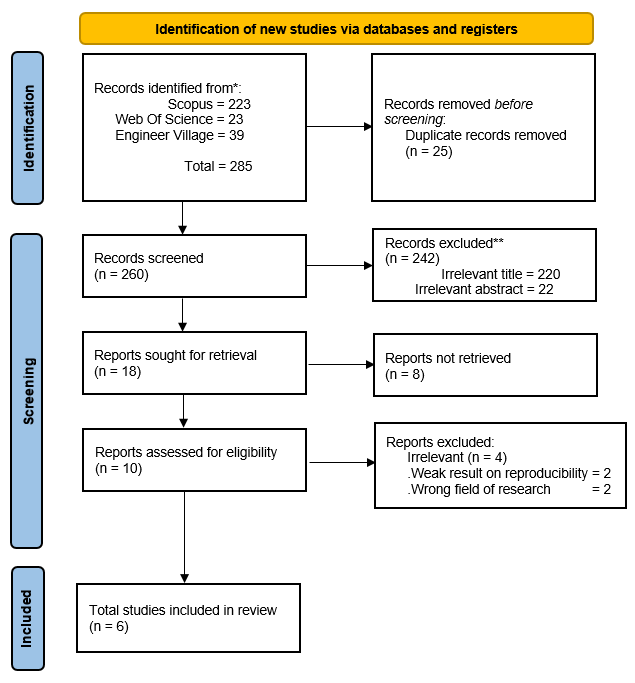
\includegraphics[width = 12cm]{chart.png}
    \caption{PRISMA flow chart }
    \label{fig:chart}
\end{figure}
\newpage

% Google scholar (Huy)
% Review paper 1
There are many articles about assessment of reproducibility of scientific researches.
In \cite{iqbal2016reproducible}, they assess the status of reproducibility and transparency in 441 biomedical journal articles published in 2000-2014. Only 1 study provided a full protocol and none made all raw data directly available. The majority of studies did not mention anything about funding or conflicts of interest. Their empirical evaluation shows that the published biomedical literature lacks transparency in important dimensions. The majority of papers claimed to present some novel discoveries, however, they suspect that very few papers truly have totally, disruptively innovative findings.

In \cite{Stagge2019Assessing}, they developed a survey tool to assess the availability of digital research artifacts published alongside peer-reviewed journal articles (e.g. data, models, code, directions for use) and reproducibility of article results.
They used the tool to assess 360 of the 1,989 articles published by six hydrology and water resources journals in 2017.
They estimated that results might be reproduced for only 0.6\% to 6.8\% of all 1,989 articles.
The survey tool identified key bottlenecks to making work more reproducible, include: only some digital artifacts available (44\% of articles), no directions (89\%), or all artifacts available but results not reproducible (5\%).
The tool can help authors, journals, funders, and institutions to self-assess manuscripts, provide feedback to improve reproducibility, and recognize and reward reproducible articles as examples for others.
% Web of Science (Thanh)

Currently, a key component of scientific communication is sufficient information for other researchers in the field to reproduce published findings. For computational and data-enabled research, this has often been interpreted to mean making available the raw data from which results were generated, the computer code that generated the findings, and any additional information needed such as workflows and input parameters. Many journals are revising author guidelines to include data and code availability. In \cite{stodden2018empirical}, the author evaluates the effectiveness of journal policy that requires the data and code necessary for reproducibility to be made available postpublication by the authors upon request. 204 scientific papers published in the journal Science were chosen, in which 44\% of chosen study and were able to reproduce the findings for 26\%. The paper presented this policy—author remission of data and code postpublication upon request—an improvement over no policy, but currently insufficient for reproducibility.


The demand for reproducible research is on the rise in disciplines concerned with data analysis and computational methods. In \cite{nust2018reproducible}, the author reviewed current recommendations for reproducible research and translated them into criteria for assessing the reproducibility of articles in the field of geographic information science (GIScience). Using this criterion, they assessed a sample of GIScience studies from the Association of Geographic Information Laboratories in Europe (AGILE) conference series, and they also collected feedback about the assessment from the study authors. Results from the author's feedback indicate that although authors support the concept of performing reproducible research, the incentives for doing this in practice are too small. Therefore, the author proposed concrete actions for individual researchers and the GIScience conference series to improve transparency and reproducibility. The available data were published in \href{https://github.com/nuest/reproducible-research-and-giscience}{this}, including the survey, programming , and evaluate data.

% Scopus (Kung)
In \cite{PAGE20188}, they explored whether the use of reproducible research practices was associated with an Systematic Review (SR) being a Cochrane review, as well as with the reported use of the Preferred Reporting Items for Systematic Reviews and Meta-Analyses statement, and they evaluated 110 SRs of therapeutic interventions, 78 (71\%) of which were non-Cochrane SRs. Across the SRs, there were 2,139 meta-analytic effects (including subgroup meta-analytic effects and sensitivity analyses), 1,551 (73\%) of which were reported in sufficient detail to recreate them. And finally Reproducible research practices are underused in SRs of biomedical interventions. Adoption of such practices facilitates identification of errors and allows the SR data to help us  reanalyzed.

Furthermore, in the article \cite{Wang2015}, the scientific community and decision-makers are increasingly concerned about transparency and reproducibility of epide-miologic studies using longitudinal healthcare databases. We explored the extent to which published pharmacoepidemio-logic studies using commercially available databases could be reproduced by other investigators.Full reproducibility in healthcare database studies occurs when independent investigators are able to apply the same design and analytic choices to the same source data, and are able to obtain the same analytic population and estimated measures of associa-tion (or at least a near exact reproduction). The scientific com-munity as a whole would benefit and the credibility of healthcare database studies would increase if greater effort were directed toward ensuring that public reporting for database studies con-tained sufficient detail to allow full reproduction. Without repro-duction there can be no replication and without replication there can be little trust in our research output.

\section{User story evaluation}
Within the fifty-four user stories of the class, the Freshman team performs a meta-analyze method to evaluate the stories. Indeed, the evaluation process contains four steps. Firstly, all stories are categorized into eight main ideas which have the same topic like the same AI web service or the same assessment the reproducibility...Secondly, the specific ideals are created by the combination of the main ideal and initial user stories. That specific ideals contain the ideal per the main ideal. In the third step, the two groups of sub-user story built by restructuring the similar ideal of the main and specific ideal. Lastly, the final six user stories were released with the merge of the above two sub-story as below:

1. As a student, I need a web service that can use a database to assess the reproducibility of the user and current article, so that I can improve my article reproducibility.

2. As a student, I need a web service that can assess the reproducibility of the article in PDF and text files, so that I can save conversion time.

3. As a student, I need a web service that can determine the article's reproducibility contributor, so that I can know the main ideas easier.

4. As a student, I need a web service that can give feedback and suggest some good reproducibility articles as references, so that I can improve my article reproducibility.

5. As a student, I need a web service that can give some suggested synonyms during the searching, so that I can improve my search result.

6. As a student, I need a web service with a user-friendly interface, so that I can use it easily.

\begin{figure}[h]
    \centering
    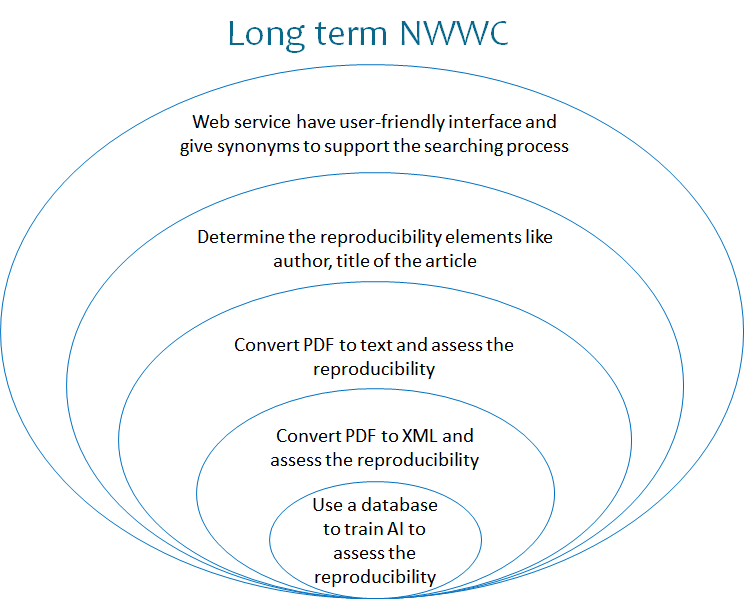
\includegraphics[width = 12cm]{Long term NWWC.png}
    \caption{Long term NWWC}
    \label{fig:Long term NWWC}
\end{figure}
\newpage


\href{https://www.dropbox.com/home/NordlingLab_Course_ScientificInformation/Team_Freshman/Literature\%20review\%20on\%20assessments\%20of\%20reproducibility}{.Data for training.}
%----------------------------------------------------------------------------------------
%	RESULTS AND DISCUSSION
%----------------------------------------------------------------------------------------

%----------------------------------------------------------------------------------------
%	BIBLIOGRAPHY
%----------------------------------------------------------------------------------------

\renewcommand{\refname}{\spacedlowsmallcaps{References}} % For modifying the bibliography heading

\bibliographystyle{unsrt}

\bibliography{technical_report.bib} % The file containing the bibliography

%----------------------------------------------------------------------------------------

\end{document}